\chapter{Resultados}
\label{cap:4-resultados}

\section{Resultados del estudio estadístico}

\begin{figure}[H]
    \centering
    \begin{subfigure}[t]{.49\textwidth}
      \centering
      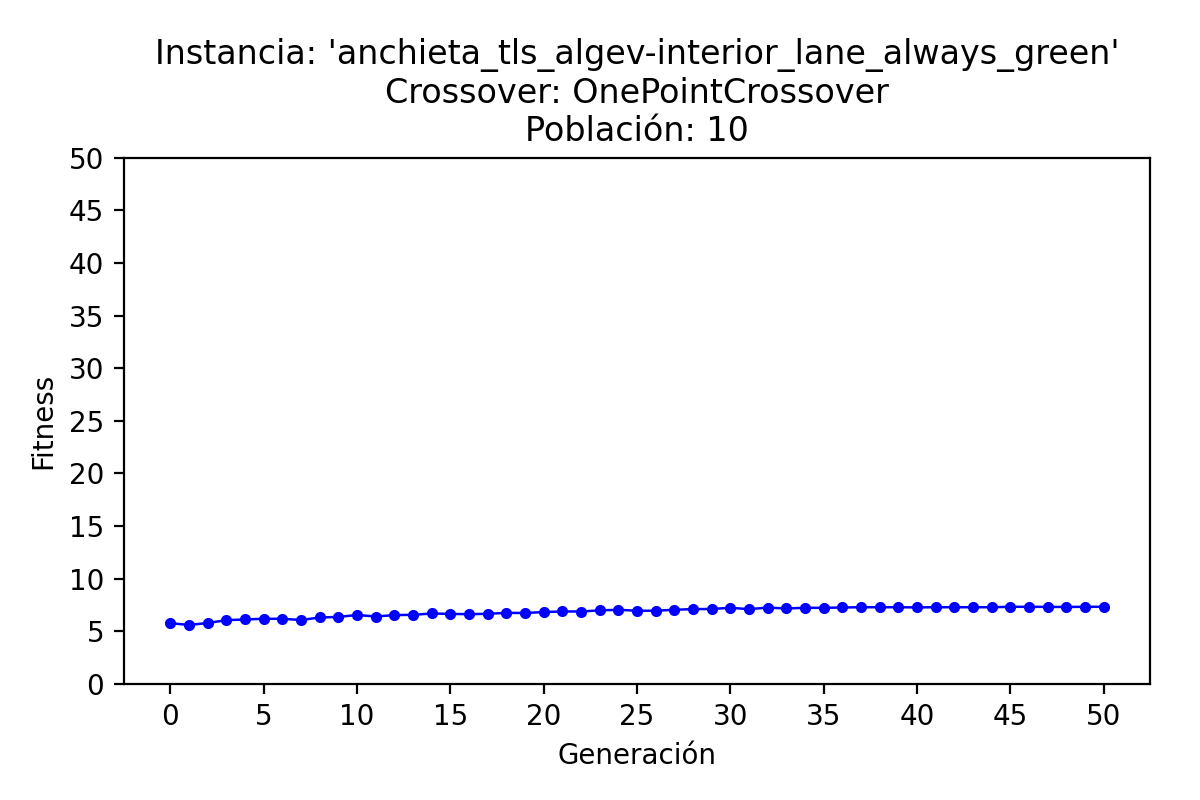
\includegraphics[width=\textwidth]{report/images/estudio/anchieta_tls_algev-interior_lane_always_green-OnePointCrossover-10.png}
    \end{subfigure}
    \hfill
    \begin{subfigure}[t]{.49\textwidth}
      \centering
      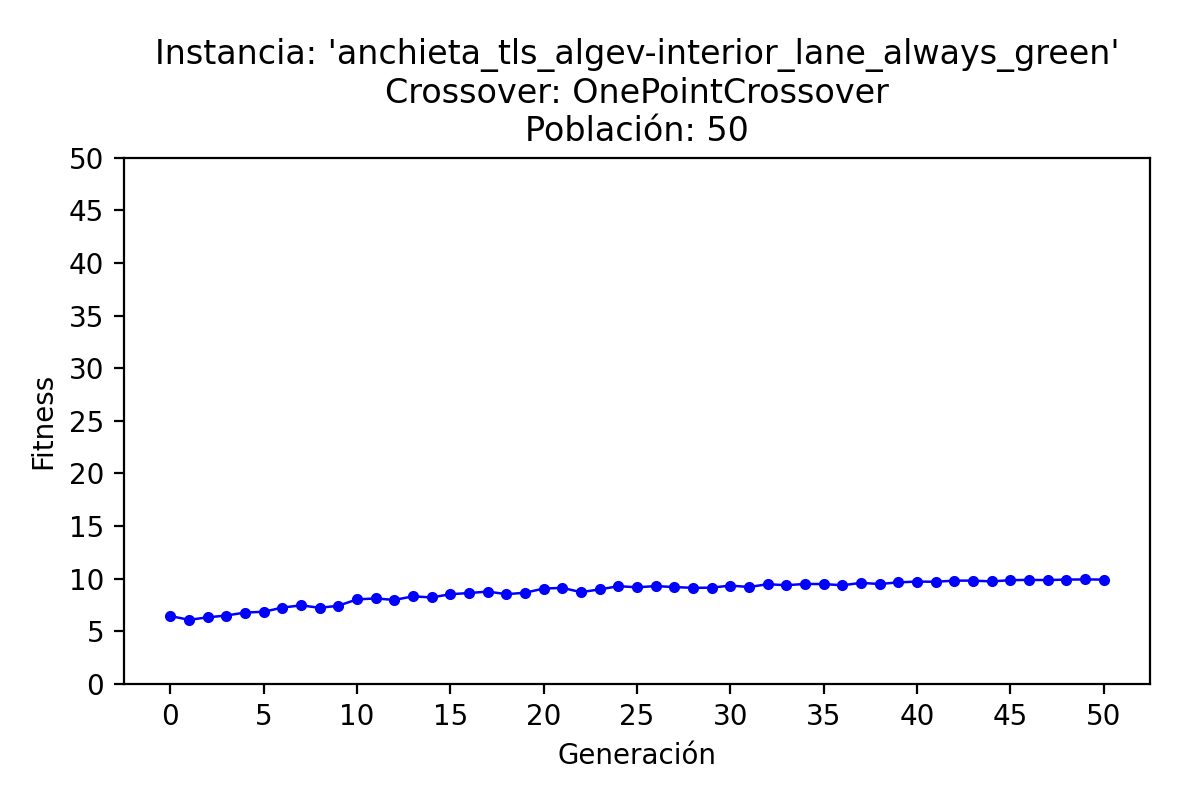
\includegraphics[width=\textwidth]{report/images/estudio/anchieta_tls_algev-interior_lane_always_green-OnePointCrossover-50.png}
    \end{subfigure}
    \vspace{0.7cm}
    \begin{subfigure}[t]{.49\textwidth}
      \centering
      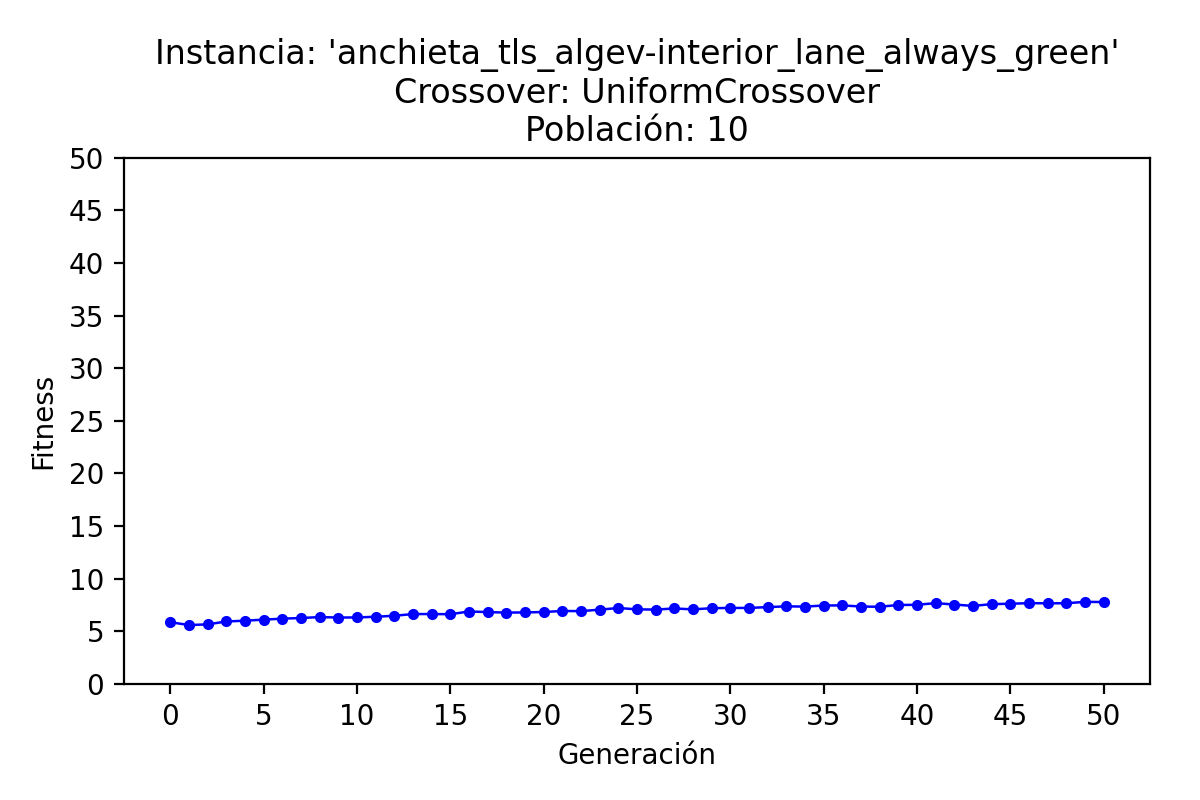
\includegraphics[width=\textwidth]{report/images/estudio/anchieta_tls_algev-interior_lane_always_green-UniformCrossover-10.png}
    \end{subfigure}
    \hfill
    \begin{subfigure}[t]{.49\textwidth}
      \centering
      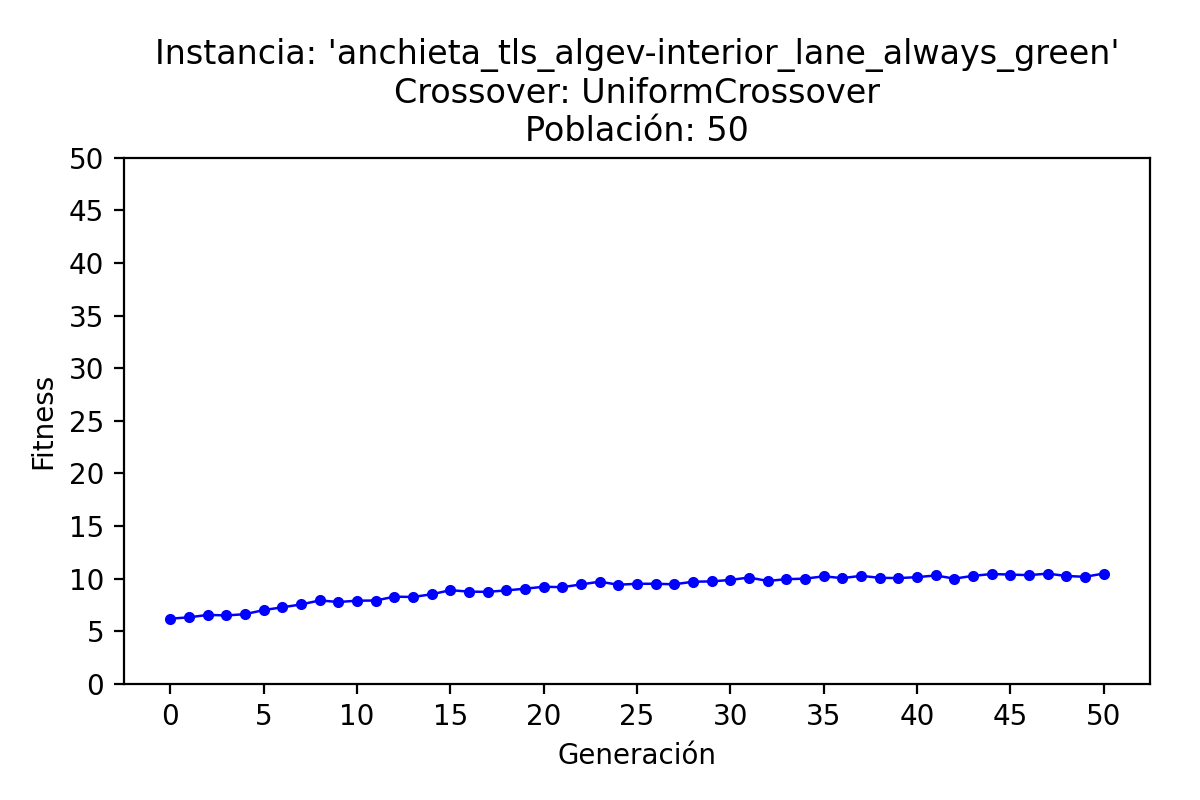
\includegraphics[width=\textwidth]{report/images/estudio/anchieta_tls_algev-interior_lane_always_green-UniformCrossover-50.png}
    \end{subfigure}
    \caption{Evolución del fitness medio entre ejecuciones del mejor candidato de cada generación para la instancia anchieta\_tls\_interior\_lane\_always\_green}
    \label{fig:estudio:anchieta_tls_interior_lane_always_green}
\end{figure}

\begin{figure}[H]
    \centering
    \begin{subfigure}[t]{.49\textwidth}
      \centering
      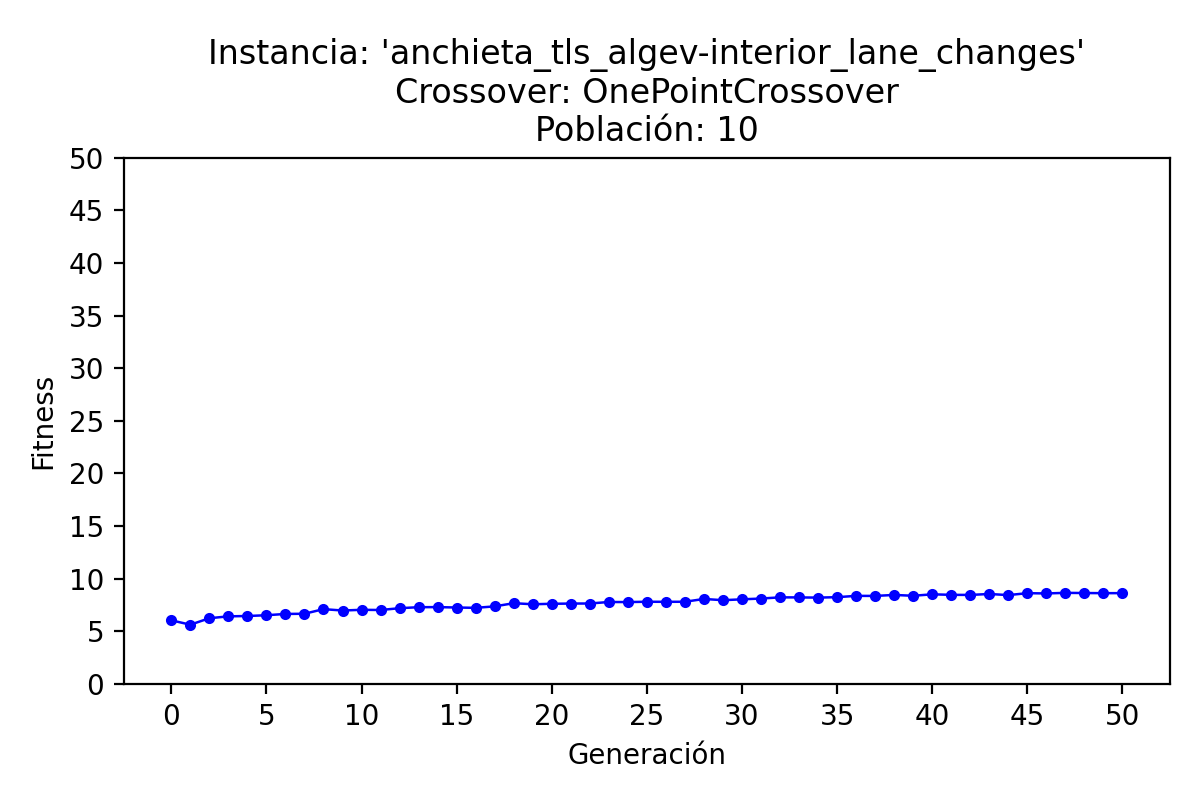
\includegraphics[width=\textwidth]{report/images/estudio/anchieta_tls_algev-interior_lane_changes-OnePointCrossover-10.png}
    \end{subfigure}
    \hfill
    \begin{subfigure}[t]{.49\textwidth}
      \centering
      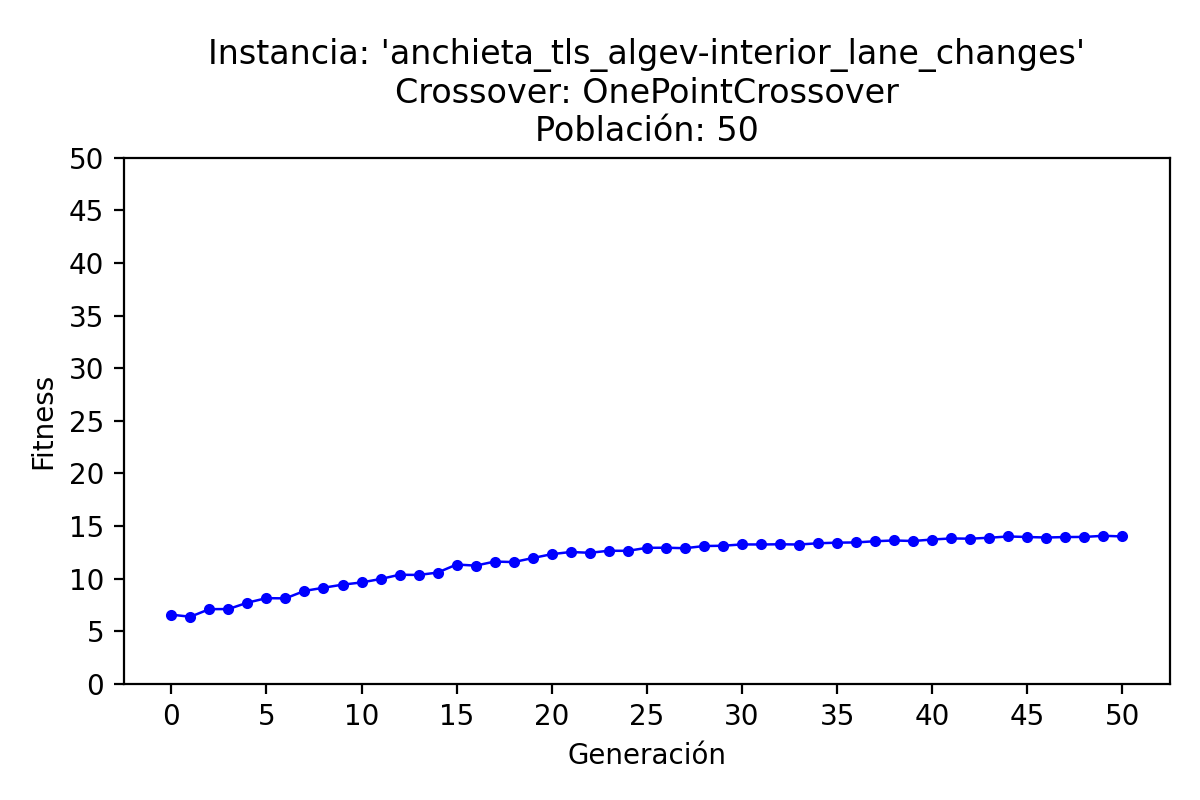
\includegraphics[width=\textwidth]{report/images/estudio/anchieta_tls_algev-interior_lane_changes-OnePointCrossover-50.png}
    \end{subfigure}
    \vspace{0.7cm}
    \begin{subfigure}[t]{.49\textwidth}
      \centering
      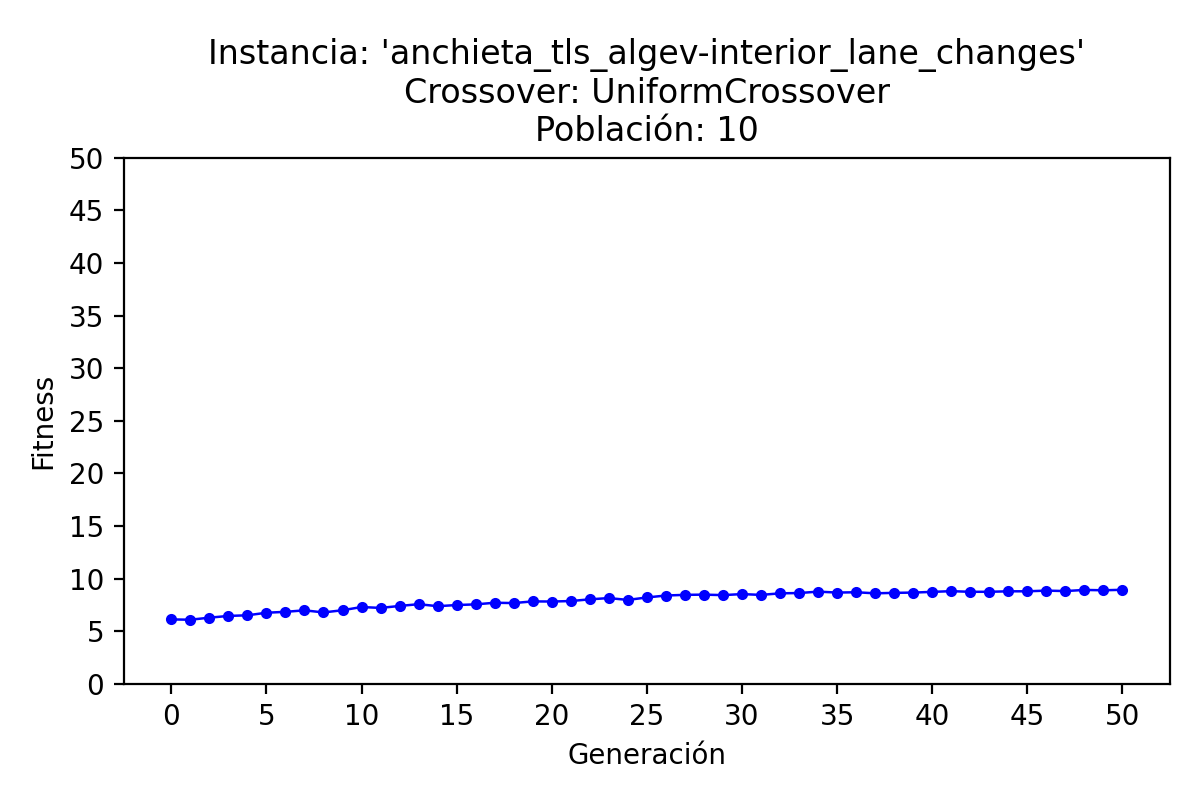
\includegraphics[width=\textwidth]{report/images/estudio/anchieta_tls_algev-interior_lane_changes-UniformCrossover-10.png}
    \end{subfigure}
    \hfill
    \begin{subfigure}[t]{.49\textwidth}
      \centering
      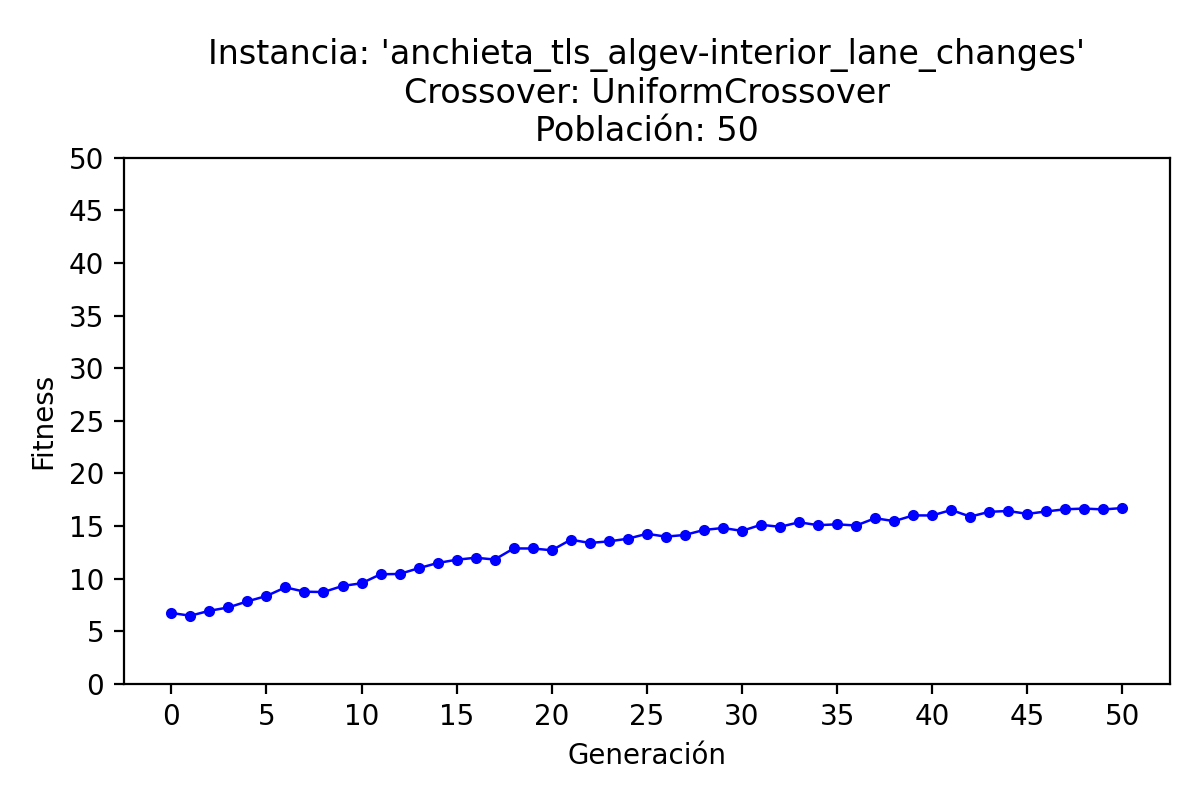
\includegraphics[width=\textwidth]{report/images/estudio/anchieta_tls_algev-interior_lane_changes-UniformCrossover-50.png}
    \end{subfigure}
    \caption{Evolución del fitness medio entre ejecuciones del mejor candidato de cada generación para la instancia anchieta\_tls\_interior\_lane\_changes}
    \label{fig:estudio:anchieta_tls_interior_lane_changes}
\end{figure}


\begin{figure}[H]
    \centering
    \begin{subfigure}[t]{.49\textwidth}
      \centering
      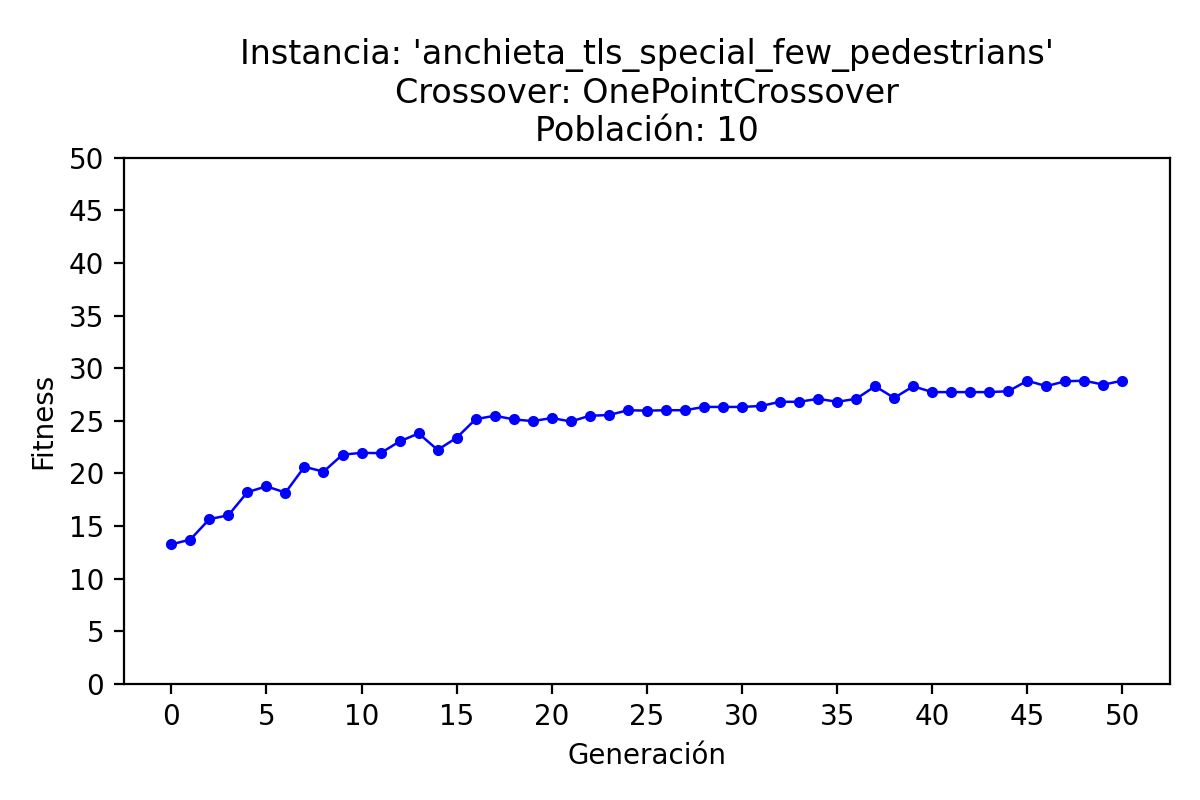
\includegraphics[width=\textwidth]{report/images/estudio/anchieta_tls_special_few_pedestrians-OnePointCrossover-10.png}
    \end{subfigure}
    \hfill
    \begin{subfigure}[t]{.49\textwidth}
      \centering
      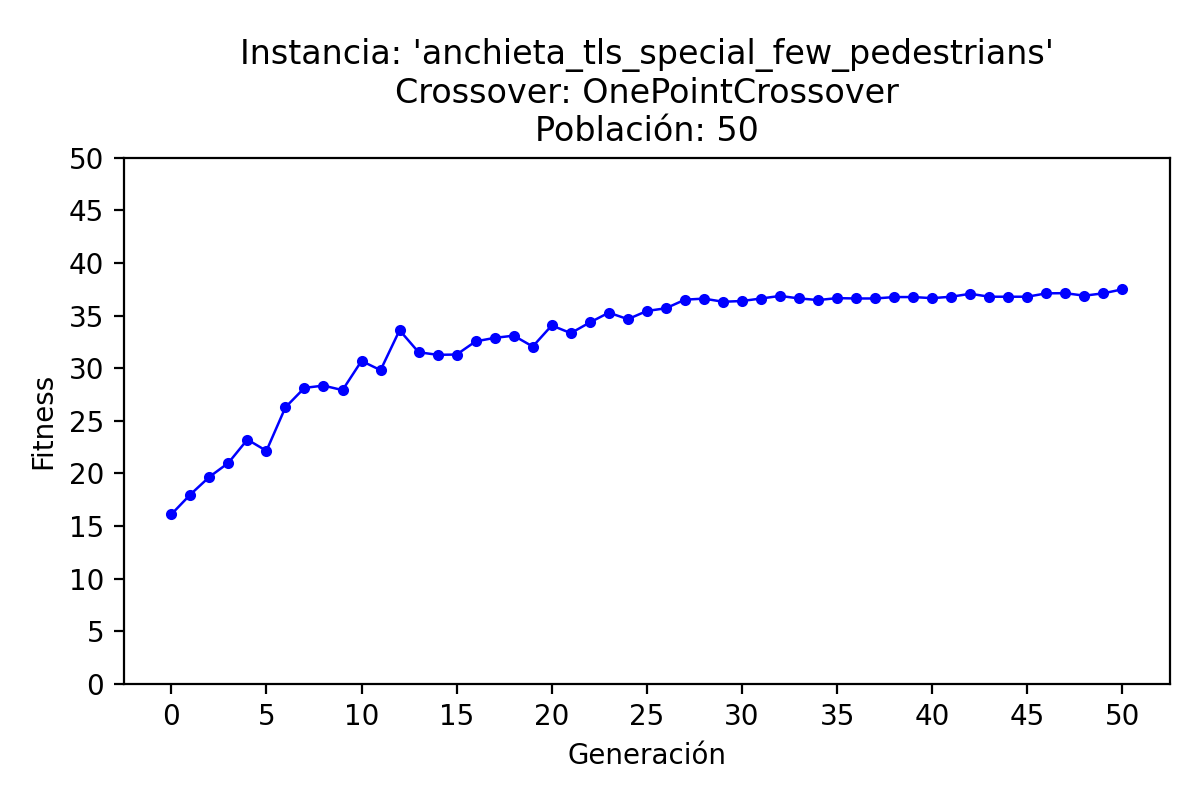
\includegraphics[width=\textwidth]{report/images/estudio/anchieta_tls_special_few_pedestrians-OnePointCrossover-50.png}
    \end{subfigure}
    \vspace{0.7cm}
    \begin{subfigure}[t]{.49\textwidth}
      \centering
      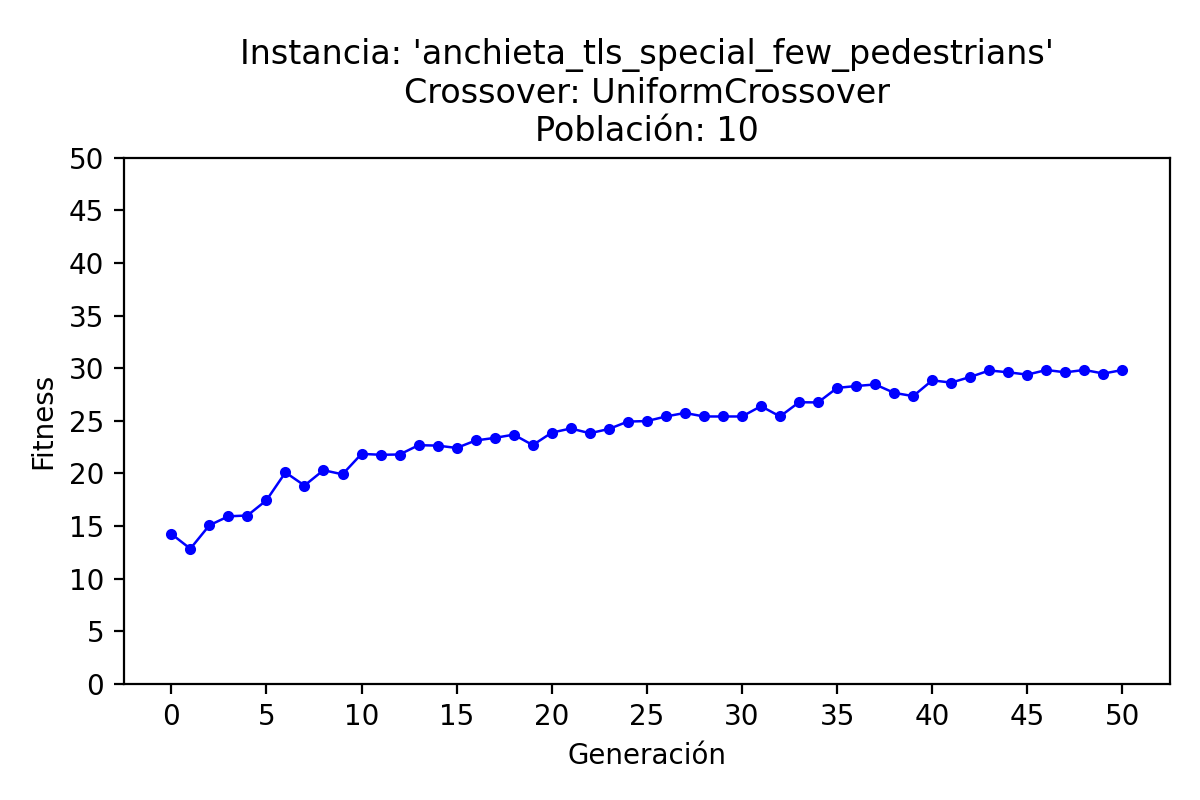
\includegraphics[width=\textwidth]{report/images/estudio/anchieta_tls_special_few_pedestrians-UniformCrossover-10.png}
    \end{subfigure}
    \hfill
    \begin{subfigure}[t]{.49\textwidth}
      \centering
      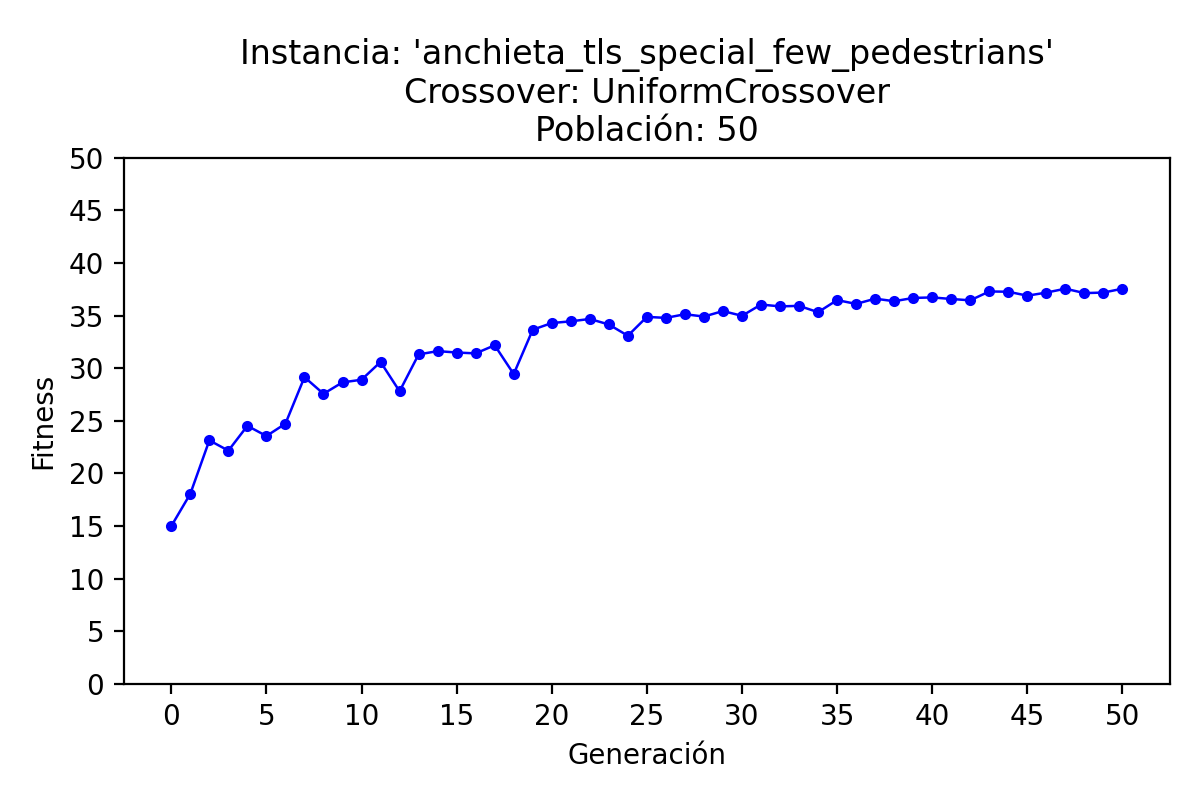
\includegraphics[width=\textwidth]{report/images/estudio/anchieta_tls_special_few_pedestrians-UniformCrossover-50.png}
    \end{subfigure}
    \caption{Evolución del fitness medio entre ejecuciones del mejor candidato de cada generación para la instancia anchieta\_no\_tls\_few\_pedestrians}
    \label{fig:estudio:anchieta_tls_special_few_pedestrians}
\end{figure}

\begin{figure}[H]
    \centering
    \begin{subfigure}[t]{.49\textwidth}
      \centering
      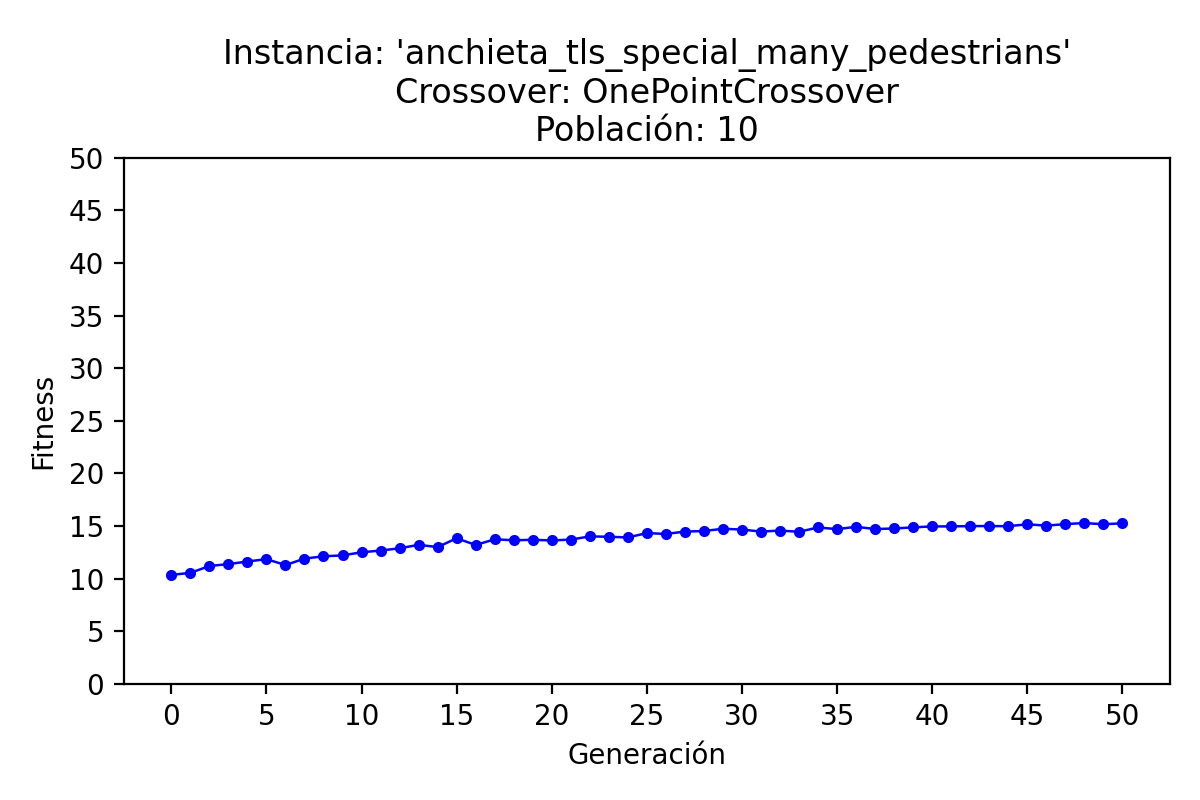
\includegraphics[width=\textwidth]{report/images/estudio/anchieta_tls_special_many_pedestrians-OnePointCrossover-10.png}
    \end{subfigure}
    \hfill
    \begin{subfigure}[t]{.49\textwidth}
      \centering
      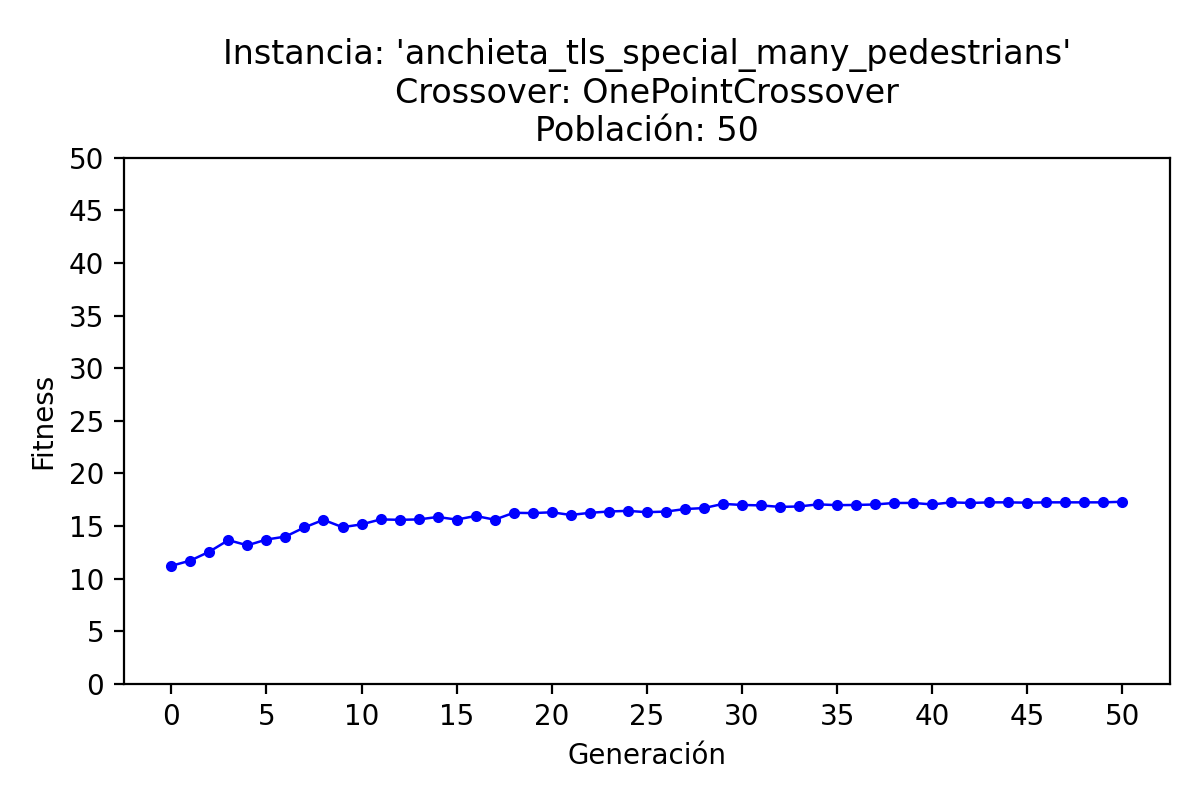
\includegraphics[width=\textwidth]{report/images/estudio/anchieta_tls_special_many_pedestrians-OnePointCrossover-50.png}
    \end{subfigure}
    \vspace{0.7cm}
    \begin{subfigure}[t]{.49\textwidth}
      \centering
      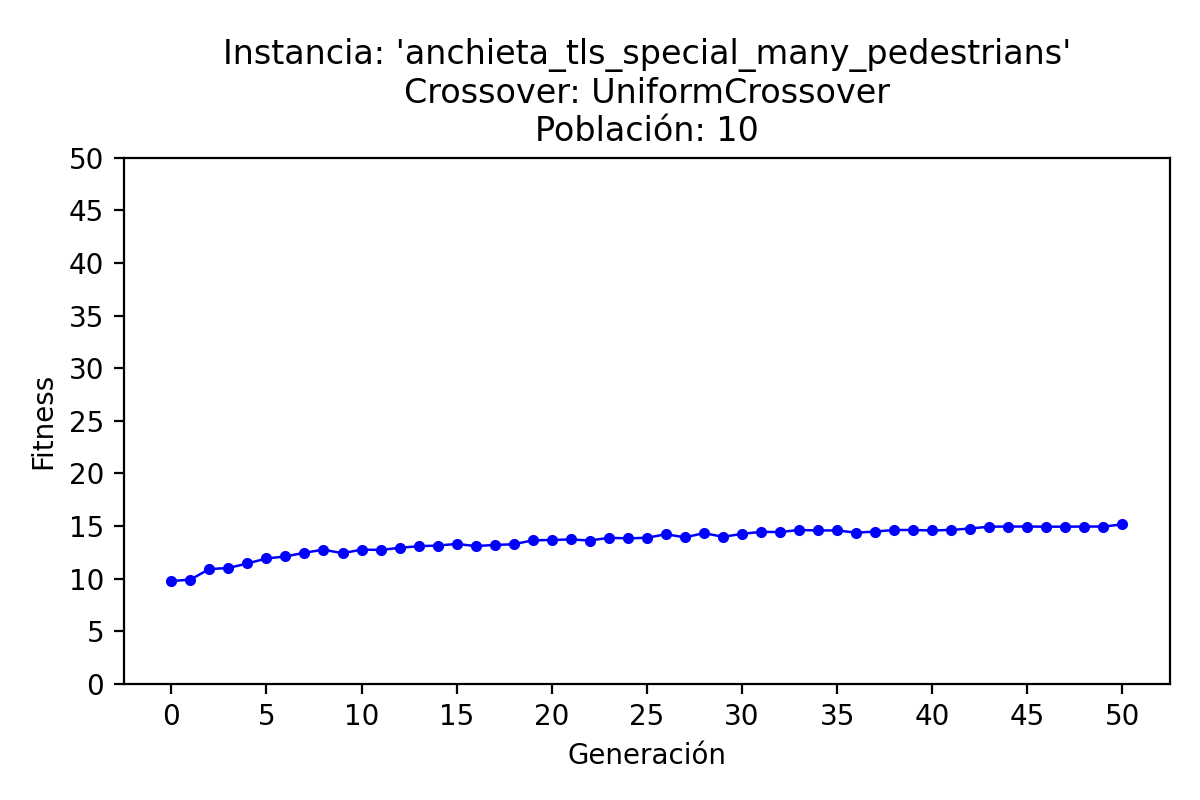
\includegraphics[width=\textwidth]{report/images/estudio/anchieta_tls_special_many_pedestrians-UniformCrossover-10.png}
    \end{subfigure}
    \hfill
    \begin{subfigure}[t]{.49\textwidth}
      \centering
      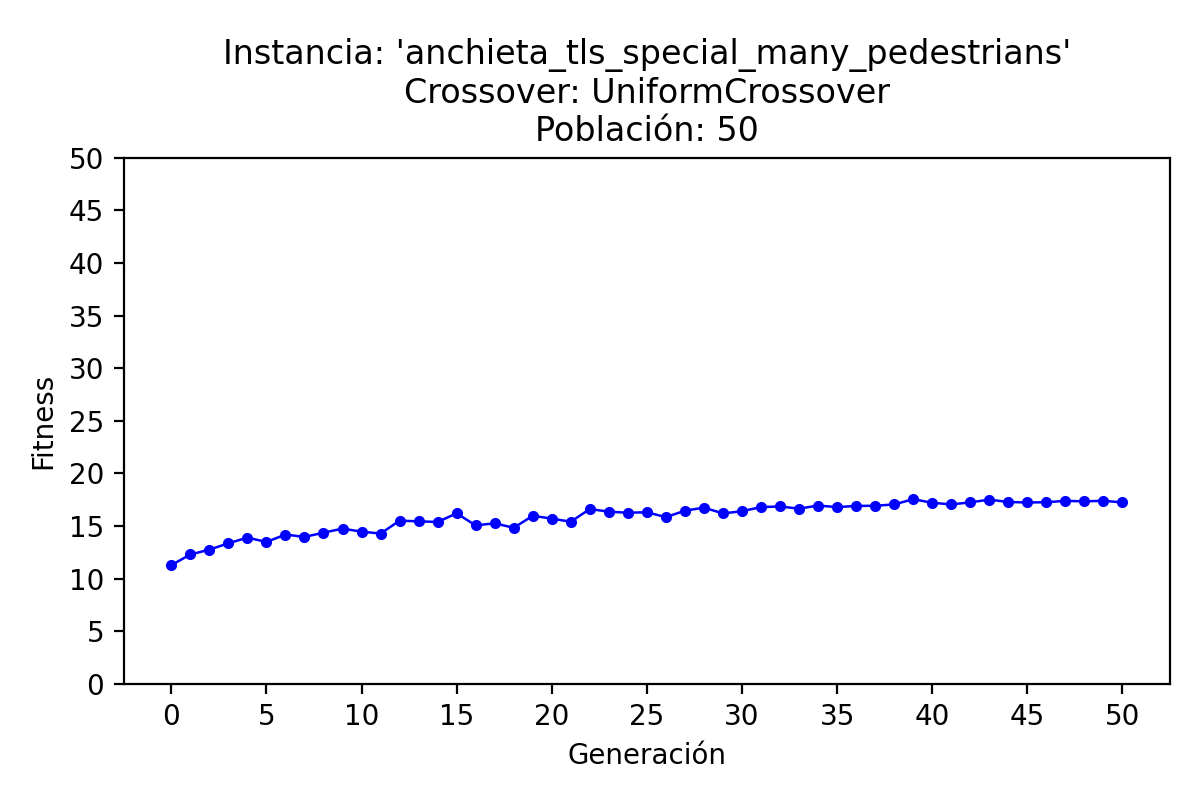
\includegraphics[width=\textwidth]{report/images/estudio/anchieta_tls_special_many_pedestrians-UniformCrossover-50.png}
    \end{subfigure}
    \caption{Evolución del fitness medio entre ejecuciones del mejor candidato de cada generación para la instancia anchieta\_no\_tls\_many\_pedestrians}
    \label{fig:estudio:anchieta_tls_special_many_pedestrians}
\end{figure}

\subsection{Resultados de la comparación de las distintas configuraciones}

\begin{table}[H]
\caption{}
\label{tab:1}
\resizebox{\textwidth}{!}{\begin{tabular}{lllllll}
\hline
\multicolumn{7}{c}{\textbf{anchieta\_tls\_interior\_lane\_always\_green}}                                                                                                                                                                                   \\ \hline
\multicolumn{1}{c}{\multirow{2}{*}{\textit{Conjuntos de parámetros 1 y 2}}}        & \multicolumn{2}{c}{\textit{Media}}            & \multicolumn{2}{c}{\textit{Mediana}}          & \multicolumn{1}{c}{\multirow{2}{*}{\textit{p-value}}} & \multicolumn{1}{c}{\multirow{2}{*}{\textit{Ganador}}} \\ \cline{2-5}
\multicolumn{1}{c}{}                                                & \multicolumn{1}{c}{1} & \multicolumn{1}{c}{2} & \multicolumn{1}{c}{1} & \multicolumn{1}{c}{2} & \multicolumn{1}{c}{}                                  & \multicolumn{1}{c}{}                                  \\ \hline
OnePointCrossover/Pop10 y OnePointCrossover/Pop50                   & 7.364113              & 9.962546              & 7.298901              & 10.05993              & 5.78933e-05                                           & OnePointCrossover/Pop50                               \\ \hline
OnePointCrossover/Pop10 y UniformCrossover/Pop10                    & 7.364113              & 7.859806              & 7.298901              & 7.632471              & 0.1928009                                             & No hay diferencia estadística                         \\ \hline
OnePointCrossover/Pop10 y UniformCrossover/Pop50                    & 7.364113              & 11.16813              & 7.298901              & 11.15414              & 0.0001570523                                          & UniformCrossover/Pop50                                \\ \hline
OnePointCrossover/Pop50 y UniformCrossover/Pop10                    & 9.962546              & 7.859806              & 10.05993              & 7.632471              & 0.0001639967                                          & OnePointCrossover/Pop50                               \\ \hline
OnePointCrossover/Pop50 y UniformCrossover/Pop50                    & 9.962546              & 11.16813              & 10.05993              & 11.15414              & 0.0101652                                             & UniformCrossover/Pop50                                \\ \hline
UniformCrossover/Pop10 y UniformCrossover/Pop50                     & 7.859806              & 11.16813              & 7.632471              & 11.15414              & 0.0001570523                                          & UniformCrossover/Pop50                                \\ \hline
\end{tabular}}
\end{table}



\begin{table}[H]
\caption{}
\label{tab:2}
\resizebox{\textwidth}{!}{\begin{tabular}{lllllll}
\hline
\multicolumn{7}{c}{\textbf{anchieta\_tls\_interior\_lane\_changes}}                                                                                                                                                                                         \\ \hline
\multicolumn{1}{c}{\multirow{2}{*}{\textit{Conjuntos de parámetros 1 y 2}}}        & \multicolumn{2}{c}{\textit{Media}}            & \multicolumn{2}{c}{\textit{Mediana}}          & \multicolumn{1}{c}{\multirow{2}{*}{\textit{p-value}}} & \multicolumn{1}{c}{\multirow{2}{*}{\textit{Ganador}}} \\ \cline{2-5}
\multicolumn{1}{c}{}                                                & \multicolumn{1}{c}{1} & \multicolumn{1}{c}{2} & \multicolumn{1}{c}{1} & \multicolumn{1}{c}{2} & \multicolumn{1}{c}{}                                  & \multicolumn{1}{c}{}                                  \\ \hline
OnePointCrossover/Pop10 y OnePointCrossover/Pop50                   & 8.654163              & 14.24831              & 8.53437               & 14.10958              & 1.21893e-06                                           & OnePointCrossover/Pop50                               \\ \hline
OnePointCrossover/Pop10 y UniformCrossover/Pop10                    & 8.654163              & 9.004224              & 8.53437               & 8.693441              & 0.6450571                                             & No hay diferencia estadística                         \\ \hline
OnePointCrossover/Pop10 y UniformCrossover/Pop50                    & 8.654163              & 17.58131              & 8.53437               & 17.49452              & 1.79459e-09                                           & UniformCrossover/Pop50                                \\ \hline
OnePointCrossover/Pop50 y UniformCrossover/Pop10                    & 14.24831              & 9.004224              & 14.10958              & 8.693441              & 2.836182e-06                                          & OnePointCrossover/Pop50                               \\ \hline
OnePointCrossover/Pop50 y UniformCrossover/Pop50                    & 14.24831              & 17.58131              & 14.10958              & 17.49452              & 0.000899443                                           & UniformCrossover/Pop50                                \\ \hline
UniformCrossover/Pop10 y UniformCrossover/Pop50                     & 9.004224              & 17.58131              & 8.693441              & 17.49452              & 3.310727e-09                                          & UniformCrossover/Pop50                                \\ \hline
\end{tabular}}
\end{table}




\begin{table}[]
\caption{}
\label{tab:3}
\resizebox{\textwidth}{!}{\begin{tabular}{lllllll}
\hline
\multicolumn{7}{c}{\textbf{anchieta\_tls\_special\_few\_pedestrians}}                                                                                                                                                                                             \\ \hline
\multicolumn{1}{c}{\multirow{2}{*}{\textit{Conjuntos de parámetros 1 y 2}}}        & \multicolumn{2}{c}{\textit{Media}}            & \multicolumn{2}{c}{\textit{Mediana}}          & \multicolumn{1}{c}{\multirow{2}{*}{\textit{p-value}}} & \multicolumn{1}{c}{\multirow{2}{*}{\textit{Ganador}}} \\ \cline{2-5}
\multicolumn{1}{c}{}                                                & \multicolumn{1}{c}{1} & \multicolumn{1}{c}{2} & \multicolumn{1}{c}{1} & \multicolumn{1}{c}{2} & \multicolumn{1}{c}{}                                  & \multicolumn{1}{c}{}                                  \\ \hline
OnePointCrossover/Pop10 y OnePointCrossover/Pop50                   & 29.45247              & 37.67554              & 27.4298               & 38.05608              & 0.0002177574                                          & OnePointCrossover/Pop50                               \\ \hline
OnePointCrossover/Pop10 y UniformCrossover/Pop10                    & 29.45247              & 29.88526              & 27.4298               & 28.53967              & 0.8623907                                             & No hay diferencia estadística                         \\ \hline
OnePointCrossover/Pop10 y UniformCrossover/Pop50                    & 29.45247              & 38.31307              & 27.4298               & 38.35384              & 0.0003900244                                          & UniformCrossover/Pop50                                \\ \hline
OnePointCrossover/Pop50 y UniformCrossover/Pop10                    & 37.67554              & 29.88526              & 38.05608              & 28.53967              & 0.00180757                                            & OnePointCrossover/Pop50                               \\ \hline
OnePointCrossover/Pop50 y UniformCrossover/Pop50                    & 37.67554              & 38.31307              & 38.05608              & 38.35384              & 0.4469909                                             & No hay diferencia estadística                         \\ \hline
UniformCrossover/Pop10 y UniformCrossover/Pop50                     & 29.88526              & 38.31307              & 28.53967              & 38.35384              & 0.001050841                                           & UniformCrossover/Pop50                                \\ \hline
\end{tabular}}
\end{table}



\begin{table}[]
\caption{}
\label{tab:4}
\resizebox{\textwidth}{!}{\begin{tabular}{lllllll}
\hline
\multicolumn{7}{c}{\textbf{anchieta\_tls\_special\_many\_pedestrians}}                                                                                                                                                                                            \\ \hline
\multicolumn{1}{c}{\multirow{2}{*}{\textit{Conjuntos de parámetros 1 y 2}}}        & \multicolumn{2}{c}{\textit{Media}}            & \multicolumn{2}{c}{\textit{Mediana}}          & \multicolumn{1}{c}{\multirow{2}{*}{\textit{p-value}}} & \multicolumn{1}{c}{\multirow{2}{*}{\textit{Ganador}}} \\ \cline{2-5}
\multicolumn{1}{c}{}                                                & \multicolumn{1}{c}{1} & \multicolumn{1}{c}{2} & \multicolumn{1}{c}{1} & \multicolumn{1}{c}{2} & \multicolumn{1}{c}{}                                  & \multicolumn{1}{c}{}                                  \\ \hline
OnePointCrossover/Pop10 y OnePointCrossover/Pop50                   & 15.3666               & 17.38808              & 15.65755              & 17.53609              & 7.402106e-05                                          & OnePointCrossover/Pop50                               \\ \hline
OnePointCrossover/Pop10 y UniformCrossover/Pop10                    & 15.3666               & 15.26587              & 15.65755              & 15.11698              & 0.86804                                               & No hay diferencia estadística                         \\ \hline
OnePointCrossover/Pop10 y UniformCrossover/Pop50                    & 15.3666               & 17.72223              & 15.65755              & 17.9043               & 4.202438e-05                                          & UniformCrossover/Pop50                                \\ \hline
OnePointCrossover/Pop50 y UniformCrossover/Pop10                    & 17.38808              & 15.26587              & 17.53609              & 15.11698              & 0.001255819                                           & OnePointCrossover/Pop50                               \\ \hline
OnePointCrossover/Pop50 y UniformCrossover/Pop50                    & 17.38808              & 17.72223              & 17.53609              & 17.9043               & 0.390172                                              & No hay diferencia estadística                         \\ \hline
UniformCrossover/Pop10 y UniformCrossover/Pop50                     & 15.26587              & 17.72223              & 15.11698              & 17.9043               & 0.0005555893                                          & UniformCrossover/Pop50                                \\ \hline
\end{tabular}}
\end{table}



\section{Resultados de la simulación}


\begin{table}[H]
\caption{}
\label{tab:my-table}
\resizebox{\textwidth}{!}{\begin{tabular}{llllllllllllll}
\hline
\multicolumn{14}{c}{\textbf{Resultados de la simulación}}                                                                                                                                                                                                                                                                                                                                                                                                     \\ \hline
\multicolumn{1}{c}{\multirow{2}{*}{\textit{Instancia}}} & \multicolumn{4}{c}{\textit{Vehículos}}                                                                                             &  & \multicolumn{6}{c}{\textit{Estadísticas}}                                                                                                                                                                            &  & \multirow{2}{*}{\textit{Fitness}} \\ \cline{2-5} \cline{7-12}
\multicolumn{1}{c}{}                                    & \multicolumn{1}{c}{Cargados} & \multicolumn{1}{c}{Insertados} & \multicolumn{1}{c}{En ejecución} & \multicolumn{1}{c}{A la espera} &  & \multicolumn{1}{c}{Longitud (m)} & \multicolumn{1}{c}{Velocidad (m/s)} & \multicolumn{1}{c}{T. perdido (s)} & \multicolumn{1}{c}{T. espera (s)} & \multicolumn{1}{c}{Duración (s)} & \multicolumn{1}{c}{Retardo (s)} &  &                                   \\ \hline
anchieta\_no\_tls                                       & 14181.8                      & 13057.8                        & 614.6                            & 1124                            &  & 1705.982                         & 22.99                               & 88.34                              & 145.44                            & 44.94                            & 70.55                           &  & 21.71                             \\ \hline
anchieta\_no\_tls\_few\_pedestrians                     & 14182.8                      & 12904.8                        & 623.4                            & 1278                            &  & 1713.93                          & 23.253                              & 91.304                             & 148.404                           & 50.476                           & 71.458                          &  & 18.85                             \\ \hline
anchieta\_no\_tls\_many\_pedestrians                    & 14182.7                      & 12878.1                        & 640.1                            & 1304.6                          &  & 1707.695                         & 23.125                              & 94.263                             & 151.237                           & 51.693                           & 80.753                          &  & 17.41                             \\ \hline
anchieta\_tls\_interior\_lane\_always\_green      & 14184                        & 11954.1                        & 761.8                            & 2229.9                          &  & 1739.027                         & 23.883                              & 145.692                            & 201.943                           & 110.81                           & 85.724                          &  & 7.50                              \\ \hline
anchieta\_tls\_interior\_lane\_changes            & 14183.6                      & 12397.3                        & 781                              & 1786.3                          &  & 1708.098                         & 23.332                              & 130.275                            & 186.185                           & 91.921                           & 95.318                          &  & 10.59                             \\ \hline
anchieta\_tls\_special\_few\_pedestrians                & 14181.7                      & 12669.1                        & 678.4                            & 1512.6                          &  & 1726.209                         & 23.32                               & 106.309                            & 163.292                           & 61.791                           & 87.167                          &  & 15.01                             \\ \hline
anchieta\_tls\_special\_many\_pedestrians               & 14183.1                      & 12699.2                        & 737                              & 1483.9                          &  & 1763.325                         & 23.436                              & 115.69                             & 173.26                            & 71.151                           & 59.275                          &  & 14.09                             \\ \hline
\end{tabular}}
\end{table}